\documentclass[10pt,letterpaper]{article}
\usepackage[utf8]{inputenc}
\usepackage{graphicx}
\usepackage{rotating}
\bibliographystyle{ecology.bst}


\begin{document}
% Add line number
\linenumbers
\modulolinenumbers[1]

% Double space
\doublespacing

\section{Title:}
\label{title}

\begin{itemize}
  \item Inferring species interactions from ecological data
  \item A quantitative comparison of methods for Inferring species interactions
  from ecological data
\item Comparing inferences for species interactions from ecological data
\item On the use of ecological data for comparing species interactions
\item Comparing methods for inferring species interactions
\item A statistical analysis of methods for inferring species interactions.
\item ?
\end{itemize}

\section{Authors*}\label{authors}

\begin{itemize}
  \item Ignasi Bartomeus
  \item Kevin Cazelles
  \item F. Guillaume Blanchet
  \item Mickaël Hedde
  \item Ignacio Morales Castilla
  \item Mathilde Besson
  \item David Beauchesne
  \item Dominique Gravel
  \item Timothée Poisot
  \item Ben Weinstein
  \item Steve Vissault
\end{itemize}

\emph{Current author order drawn from a multinomial distribution, which,
ironically, might be the only acceptable use case for this distribution in this
manuscript.}

\emph{Target Journals}: Methods in Ecology and Evolution, Ecological Monographs,
Annual Review of Ecology, Evolution, and Systematics.

\section*{Abstract}
\label{abstract}

\section*{Introduction}
\label{introduction}

Biotic interactions form the backbone of biodiversity
\cite{bascompte_plant-animal_2007}. Understanding the strength, direction, and
symmetry of species interactions provides insights into the maintenance of
assemblages and potential threats from anthropogenic change. Combined with
abiotic factors, biotic interactions constrain the distributions of species,
shape the evolution of phenotypes, and influence the stability of natural
systems \cite{schleuning_predicting_2015}. A common tool for understanding
interaction are ecological networks, in which each species (nodes) are connected
based on the strength and direction of interactions (links)(Jordano 1987).
Documenting and analyzing these networks is essential to better understand the
rules underlying pairwise species interactions (Bascompte et al. 2006),
quantifying ecosystem functioning (Thomson et al 2012), and predicting the
biodiversity consequences due to anthropogenic change (ref).

The foremost requirement for species interactions is species co-occurrence,
which is itself driven by species traits through environmental filtering and
local adaptation (Hillerislambers, Mayfield, but see Kraft). Knowing where
species are located gives us insights into the interactions they may have, but
to more deeply understand the mechanisms that influence the relationships among
species, traits are necessary. As such, species traits are at the core of
biological interactions (Bartomeus et al. 2016). Here, we defined traits as
phenotypic or genotypic adaptations, that may vary through time, to exploit
abiotic or biotic resources. Note that this definition indirectly include
phylogeny as a form of trait. From this definition, conceptually, if species
co-occur, we assume that they may interact only if their respective traits
promote the efficiency of resource extraction. When traits are represented by
phylogenetic information, it is the evolution history that constrains trait
evolution either directly through phylogenetic conservatism or indirectly
through exposure to similiar environmental conditions (Graham and Wiens 2005).

In practice, the traits promoting species co-occurrence and interaction may be
hidden from us, either because they were not sampled or due to their complexity.
In such cases, co-occurrence of species is used as a proxy for interaction.
Given the correlations in occurrence or abundance of species across space or
through time, co-occurrence based methods attempt to circumvent trait-based
models by assuming species that consistently co-occur, and whose populations
co-vary, may have important biotic interactions. In this context, co-occurrence
based methods are used to describe the potential relationships species may have
while trait-based models consider the mechanisms promoting interactions.

In spite of increasing efforts, it is unlikely that ecologists will empirically
document the enormous number of interactions existing in nature
(Morales-Castilla et al. 2015). Therefore, complementing fieldwork with models
of species interactions is a promising avenue for understanding the complexity
of the natural world (ref). While direct inference is often preferable, many
interactions are rare, infrequent, or impossible to detect through human
observation. Model-based inference for ecological networks provides three
important aspects to characterize species interactions, 1) it establishes
mechanistic relationships among species, 2) it estimates uncertainty given
empirical observation, and 3) it provides an avenue to predict future
interactions. We follow Poisot (2015) and Cazelles (2016) in formulating our
general conceptual model of species interactions (Figure \ref{fig:concept}).
There is a pool of true interactions, a metaweb, in which individuals of
different species co-occur resulting in interactions among species. Any given
observation we make on this metaweb is an attempt to recover the relationships
among species using empirical data. Based on these data, model(s) are built to
characterize and elucidate the relationships among species. Some models rely
exclusively co-occurrence of individuals of different species at particular
locations and may also include information on phylogenetic history and species
traits. These models can than be used to predict the interactions among observed
species, given an uncertainty due to the spatial and/or temporal stochasticity
of the interactions. With these models it is also possible to define new
networks, based on the presence of new species in the assemblage. From these
predictions, we can estimate structural network properties such as connectance
and nestedness, while simultaneously propagating our uncertainty throughout the
analysis. In this paper, we reviewed the methods proposed to build models of
species interactions, emphasizing each method's utility for predicting the
position of a novel species in the network.

From this conceptual framework, we can decide on a set of optimal criteria to
compare existing approaches. While it is unlikely that any single method meets
all our expectations, by defining a set of standards, we can more transparently
judge the relative merits of each method to reach particular goals. The most
important aspect of a method is for it to generate accurate prediction of the
links among co-occurring species based on an estimated probability of
interaction. This prediction should come with a statement of uncertainty
regarding our confidence in parameter estimates based on empirical data. An
ideal method would also be able to make reasonable assumptions about the
interdependence of observations, and be insensitive to low sampling effort. The
mechanism determining the links among species should be clear and grounded in
ecological theory such that we can use our method to make a prediction about the
placement of a new species in the network based on a fitted model.

\section*{Methods}\label{methods}

One goal of this paper is to frame the different techniques used to model
ecological networks within a conceptual framework that would allow ecologists to
efficiently choose which technique to use with regard to various properties of
the methods and the type of ecological questions they can answer. A way to
assess the different properties of the modelling techniques is to compare them
based on specific criteria. We defined three criteria, formulated as questions,
that can be used to qualitatively compare the methods used to model ecological
networks: 1) Can the method account for the uncertainty in species
observations?; 2) Does the method provide ecological mechanisms to infer the
probability of species interactions?; and 3) Can the method be used to predict
an novel interaction?

In addition to qualitative comparison, we also provide a quantitative comparison
of methods for inferring species interactions. From a quantitative perspective,
we are interested in methods that: 1) accurately reflect the true underlying
relationships among species, 2) are insensitive to sampling effort, and 3) make
reasonable assumptions about the interdependence of species observations. To
quantitatively compare the different methods, we used simulated and reference
empirical data to establish benchmarks that will later be used to compare the
accuracy and sensitivity of currently proposed methods.

\subsection*{Modelling ecological networks - A diversity of methods}
\label{models-of-species-interactions}

When modelling ecological networks, there are different types of methods that
have been proposed in the litterature. In this section, we presented the
different techniques and group them based on their properties.

\subsubsection*{Co-occurrences models}
\label{regression-based-models}
%%% Regression-based models on co-occurrences subsubsection will probably have to be moved somewhere else to follow the structure of the Introduction where traits and phylogeny related methods are discussed firsts and co-occurrence methods are discussed later.

The simplest model of that can be designed to characterize the co-occurrence
patterns between species $i$ and $j$ in matrix $Y$ can be defined as follow

\begin{equation}
  \label{eq:coOccSimple}
  Y_{i,j} = \rho_{i,j}
\end{equation}

where the probability of interaction among species $i$ and $j$ is a fixed value
($\rho_{i,j}$). Using empirical data, we might try to estimate this value by
dividing the number of observations by the total number of observations for any
pair of species. While this is straightforward, it is insufficient because it
contains no estimate of uncertainty. The estimate is given without any
consideration for the variance due to sampling, environmental, spatial or
temporal stochasticity. This model is overly simple. By assuming that
observations are randomly drawn from a statistical distribution with parameter
$\rho_{i,j}$, we obtain a simple model that account for sampling stochasticity
in the data.

\begin{equation}
  \label{eq:coOccBern}
  Y_{i,j} \sim \text{Bernoulli}(\rho_{i,j})
\end{equation}

In equation \ref{eq:coOccBern}, we used a Bernoulli distribution, which assumes
that $Y_{i,j}$ is either 0 or 1. If $Y_{i,j}$ includes other types of data (e.g.
counts or weights) other distributions may be used instead. From equation
\ref{eq:coOccBern}, we can now estimate the probability of interaction while
accounting sampling stochasticity. Although this model is more informative than
the one presented in equation \ref{eq:coOccSimple}, it is still unsatisfying
because it depends wholly on species identity and uses no ecological theory or
inference; in short it is not mechanistic. Therefore, it is difficult to ascribe
meaning to the species association that could be highlighted by this model, or
understand how they might change in the future. In addition, from this model, we
cannot make a prediction about potential new species.

To make our model more ecologically relevant, we might add covariates $X_{i,j}$
that influence the relationship among a pair of species

\begin{equation}
  \label{eq:coOccCov}
  Y_{i,j} \sim \text{Bernoulli}(\rho_{i,j})
  \text{logit}(\rho_{i,j}) = \alpha_{i,j}+\beta_{i,j}X_{i,j}
\end{equation}

where $\beta_{i,j}$ is a regression coefficient and $\alpha_{i,j}$ is the model
intercept. In equation \ref{eq:coOccCov}, a link between species $i$ and $j$ is
a Bernoulli trial with a probability of success $\rho_{i,j}$. The probability of
success will vary based on some ecological principle ($x_{i,j}$) such as the
similarity in functional traits among species $i$ and $j$:

%%% GB: I am not sure if this equation is right... Need to check carefully.
\begin{equation}
  \label{eq:coOccTrait}
  x_{i,j}= f(\text{Trait}_i,\text{Trait}_j)
\end{equation}

%%% ICI %%%

A variety of trait-matching functions may be biologically plausible. For
example, the absolute value of the difference between traits (e.g. \(|trait_i -
trait_j|\)) or a binary difference (e.g. \(trait_i > trait_j\)), could be used
to predict which species may interact. Alternatively, the covariate may
represent the phylogenetic relatedness of species, or their relative response to
a given environmental variable.In some cases, we cannot provide a simple
trait-matching function (eg V), but must use a statistical tool to infer the
best possible combination of traits among co-occurring species that predicts
interactions. Machine learning tools provide an ideal compliment to traditional
linear models when we cannot anticipate the combinations of traits that can
influence species interaction rates. Unsupervised learning tools, such as random
forests, can give us the associations among species given a set of complex
traits. Regardless of the exact form of regression, this framework satisfies two
important goals: it allows for estimates of uncertainty in species interactions,
and it provides a mechanism shaping the probability of an interaction.

So far, we have only captured the uncertainty in the process model, the inherent
temporal or spatial stochasticity in our ecological process of interest (Hooten
and Hobbs). We may need to also account for the uncertainty in the observation
model, the ability to detect interactions given that they occur. The separation
of the observation and process model translates our ecological mechanism into
specific predictions about empirical data. For binary networks, one
straightforward way to account for the observation of interactions is to model
the detectability of network interactions.

eq iv.

\[ Y_{i,j,k} \sim Bernoulli(\phi_{i,j})\] \[ \phi_{i,j} = \omega_{i,j} *
z_{i,j}\] \[z_{i,j} \sim Bernoulii(\rho_{i,j})\] \[ logit(\rho_{i,j}) =
\alpha_{i,j} + \beta_{i,j} * x \]

Where the observation of a link between species i and species j at time k is a
Bernoulli trial with a probability \(\phi_{i,j}\), which is the outcome of the
detectability of an interaction (\(\omega_{i,j}\)) and the latent state
(\(z_{i,j}\)). This latent state is the true, but unobserved, existence of a
link, as predicted by our ecological mechanism of interest (see eq IV). Our
ability to detect this latent state depends on the detectability of an
interaction (\(\omega_{i,j}\)). The benefit of this approach is that
differentiates the probability of detection from the probability of occurrence.
Importantly, because we have explicitly defined some temporal window (k),
interactions with different levels of sampling effort can be directly compared.

\subsubsection*{Logic-based methods}\label{logic-based-methods}

{[}Ben Weinstein: For someone to fill in.{]}

\subsubsection*{Occurrence-based methods}\label{occurrence-based-methods}

{[}Ben Weinstein: For someone to fill in.{]}

\subsubsection*{Non-parametric methods}\label{non-parametric-methods}

The above methods are model based, that is, they largely use parametric
distributions to estimate the likelihood of the data given estimated model
parameters. An alternative approach is to use multivariate statistics to create
association matrices. One such method is called fourth-corner analysis, which is
a type of three table ordination (sometimes called `RLQ' analysis) (Doledec
1996). In bipartite networks, fourth-corner analysis relates the matrix of
species interactions to a matrix of traits from one level (e.g.~plants) to
another level (e.g.~pollinators) via the matrix of species innteractions (Dray \&
Legendre, 2008). This produces a correlation matrix, which is then compared to a
null expectation through matrix randomization. Randomization is a familiar tool
in network ecology, in which permuatation rules are used to compare the observed
test statistic (e.g the correlation among species occurrences) to a null
distribution based on some matrix constraint. Common constraints include the
mantainance of row sums, column sums, or other all marginal values, such that
only the identity of partners are switched. After each permutation, the test
statistic is recalulcating, yielding a null distribution. By comparing whether
the observed test statistic falls within the upper or lower 5th quantile of the
null distribution, studies distinguish whether their results could have been
generated at random given their sampling effort.

\subsection*{Quantitative comparisons}\label{quantitative-comparisons}

-\textgreater{} results: - cross comparison \textbar{} real and simulated data -
-sensitivity \textbar{} - interpretation of probabilities - method description
-for comparison

\section*{Results}\label{results}

\section*{Discussion}\label{discussion}

\subsection*{Perspectives}\label{perspectives}

\begin{itemize} \item guidelines \item challenges \item next steps \end{itemize}

\subsection*{On the virtue of prediction of species
interactions.}\label{on-the-virtue-of-prediction-of-species-interactions.}

In a context where novel ecosystems arise as a result of species invasions or
due to geographic shifts tracking climate change, our ability to predict future
interactions will limit how efficiently we anticipate and respond to threats on
biodiversity (i.e.~species local extinctions) and on humans (i.e.~spread of
infectious disease or plagues affecting to crops).

\emph{{[}Ben Weinstein: Previous text from Nacho:{]}} Indeed, on the quest for
describing species interactions, traits had played a pivotal role and several
methods have recently emerged to test hypotheses of trait matching for pairwise
interactions (Stang et al 2006, Dehling et al. 2014, Bartomeus et al 2016) or
understand the phylogenetic structure of ecological networks (Rezende et al.
2007). However, generating biological meaningful predictions of species
interactions and its emerging properties have proven challenging (Olito and Fox
2014). An ideal method is grounded in ecological theory, which makes the
description of ecological interactions interpretable. This method should be able
to not only describe, but also predict ecological interactions based on a set of
simple parameters. Importantly, this predictions should be accompanied by an
associated uncertainty. In addition, given the difficulty of empirically
assessing complete interaction networks, this method should be also robust to
the use of incomplete data. There is an urgent need to better understand how
communities interact and predict new interactions which will inevitably occur as
a result of human induced rapid environmental change. In addition, our
understanding of how species interact is limited to the few interactions are
directly observable such as pollination of predation, but key species
interactions not directly observable remains unlocked. Interactions inferences
may be the only option for describing and predicting interactions in soil food
webs or bacteria-phage networks. Finally, traits also relate to the fitness
effects gained by both interaction partners. This can potentially establish a
link with to modern coexistence theory. In fact, neutral expectations
postulating that species abundances are the main drivers of interactions, are
not incompatible with the underlying role of species traits shaping species
abundances via effects in fitness (Bartomeus et al. 2016).

\section*{Literature cited}\label{literature-cited}

\bibliography{referencesNew}

\section*{Boxes}\label{potential-boxes}

\subsection*{Soil ecology}\label{soil-ecology}

A handful of soil is the home of countless number of organisms. Soils host about
the quarter of Earth biodiversity (Decaëns et al 2006) and is recognised as the
third biotic frontier (André et al 1994). But three crucial points arise when
dealing with soil biodiversity and soil biotic interactions, (i) it is hard to
observe organisms without destroying their habitat, (ii) most of soil organisms
are tiny and cannot be bred or manipulated and (iii) soil organisms are prone to
a “Linnean deficit”. Biotic interactions in soils are shaped by soil
specificities that lead to an intense entanglement of trophic and non-trophic
interactions. For instance, soils are physically structured by the activity of
ecosystem engineers (earthworms, termites, ants, roots) that modifies, by their
own niche construction, the accessibility to resources for other soil organisms
(Jones et al 1994).

Body size of soil organisms ranges from nanometric scale (phage, bacteria) to
decimetric one (earthworms, moles, etc), leading to nested home ranges. Soils
are highly organized environments (in the three dimensions and in time). This
permits high level of niche segregation (to diminish competition) and numerous
way to escape from predators. On the most famous example of soil trophic network
comes from short grass meadows in Colorado (Hunt et al. 1987), in which nodes
were a mix of taxa, feeding guilds and pools of organic matter. The observation
of soil species interactions is hard and interaction can be inferred by various
ways. In the case of trophic interaction, this can be achieved through, for
example, gut content analyses (observation-based or DNA-based), (bio)chemical
analyses (eg PLFA, stable isotopes content), predator-prey body size
relationship, co-occurrence analysis, machine learning or a combination of them
(Digelet al 2014). Given the lack of knowledge on microbes’ biology and ecology,
co-occurrence is often interpreted as interaction (Barberan et al 2012).
Conversely to the green-world hypothesis (predator limitation of herbivores can
cascade to facilitate plant growth), soil food webs are assumed to be bottom-up
controlled detritus-based communities, but yet the ecosystem role of predators
in detrital food webs is less explored. Models of energy fluxes through soil
trophic networks remains rare (de Vries et al 2013), and nutrient cycling is
generally ignored while connecting above and belowground trophic networks (Zou
et al 2016). Hence, soil food webs studies are mainly descriptive and have poor
predictive ability.

Given the importance of plant for humankind, it is crucial to understand the how
multiple interactions control plant production for food, fibre and wood. Soils
are the place of numerous symbiotic relationships between plants and bacteria
(eg Rhizobia) or fungi (mycorrhiza). The soil microbial loop an example of
hypothesis that links multiple partners of the rhizospheric microbial food web
to explain protozoa (predators) effects on plant growth. As carbon-rich root
exudates (high C to N ratio) are continuously released into the plant
rhizosphere, those soil bacteria that consume the exudates need other sources of
nitrogen to support their growth. It is suggested that the bacteria therefore
increase their assimilation of indigenous soil organic nitrogen. When protozoa
subsequently consume the bacteria, part of this nitrogen will be released into
the soil inorganic nitrogen pool, which will increase the nitrogen pool
available for plant uptake. It has also been demonstrated that signal molecules
emitted by invertebrates can mediate plant growth and plant disease immunity
(resistance or recovery). Interactions between soil organisms and roots also
shape the plant community assembly and the aboveground trophic interactions, up
to fourth levels (plant-herbivore-parasite-parasitoïd).

Recently, DNA-based approach has been democratised to study co-occurrence of
cryptic interactions like Ericaceous plant-fungus symbioses (Toju et al 2016),
earthworm-gut bacteria symbioses (Moller et al 2015) or predator-prey
interactions (Bohan xxx). The tremendous development of next-generation DNA
sequencing will surely provide the most comprehensive and accurate measure of
trophic links in ecosystems, regardless of the size of organisms and without a
priori on the species consumed by a given organism, by matching sequences
amplified from the gut content to wide gene databases (Pompanon et al. 2012).
Finally, the integration of biogeography and network theory will yield important
results and further our understanding and forecasting ability of species
interactions, in a context of global changes.

\subsection*{Climate changes and alien species}
\label{climate-changes-and-alien-species}

\subsection*{Community/evolution ecology}
\label{communityevolution-ecology}

\begin{figure}
  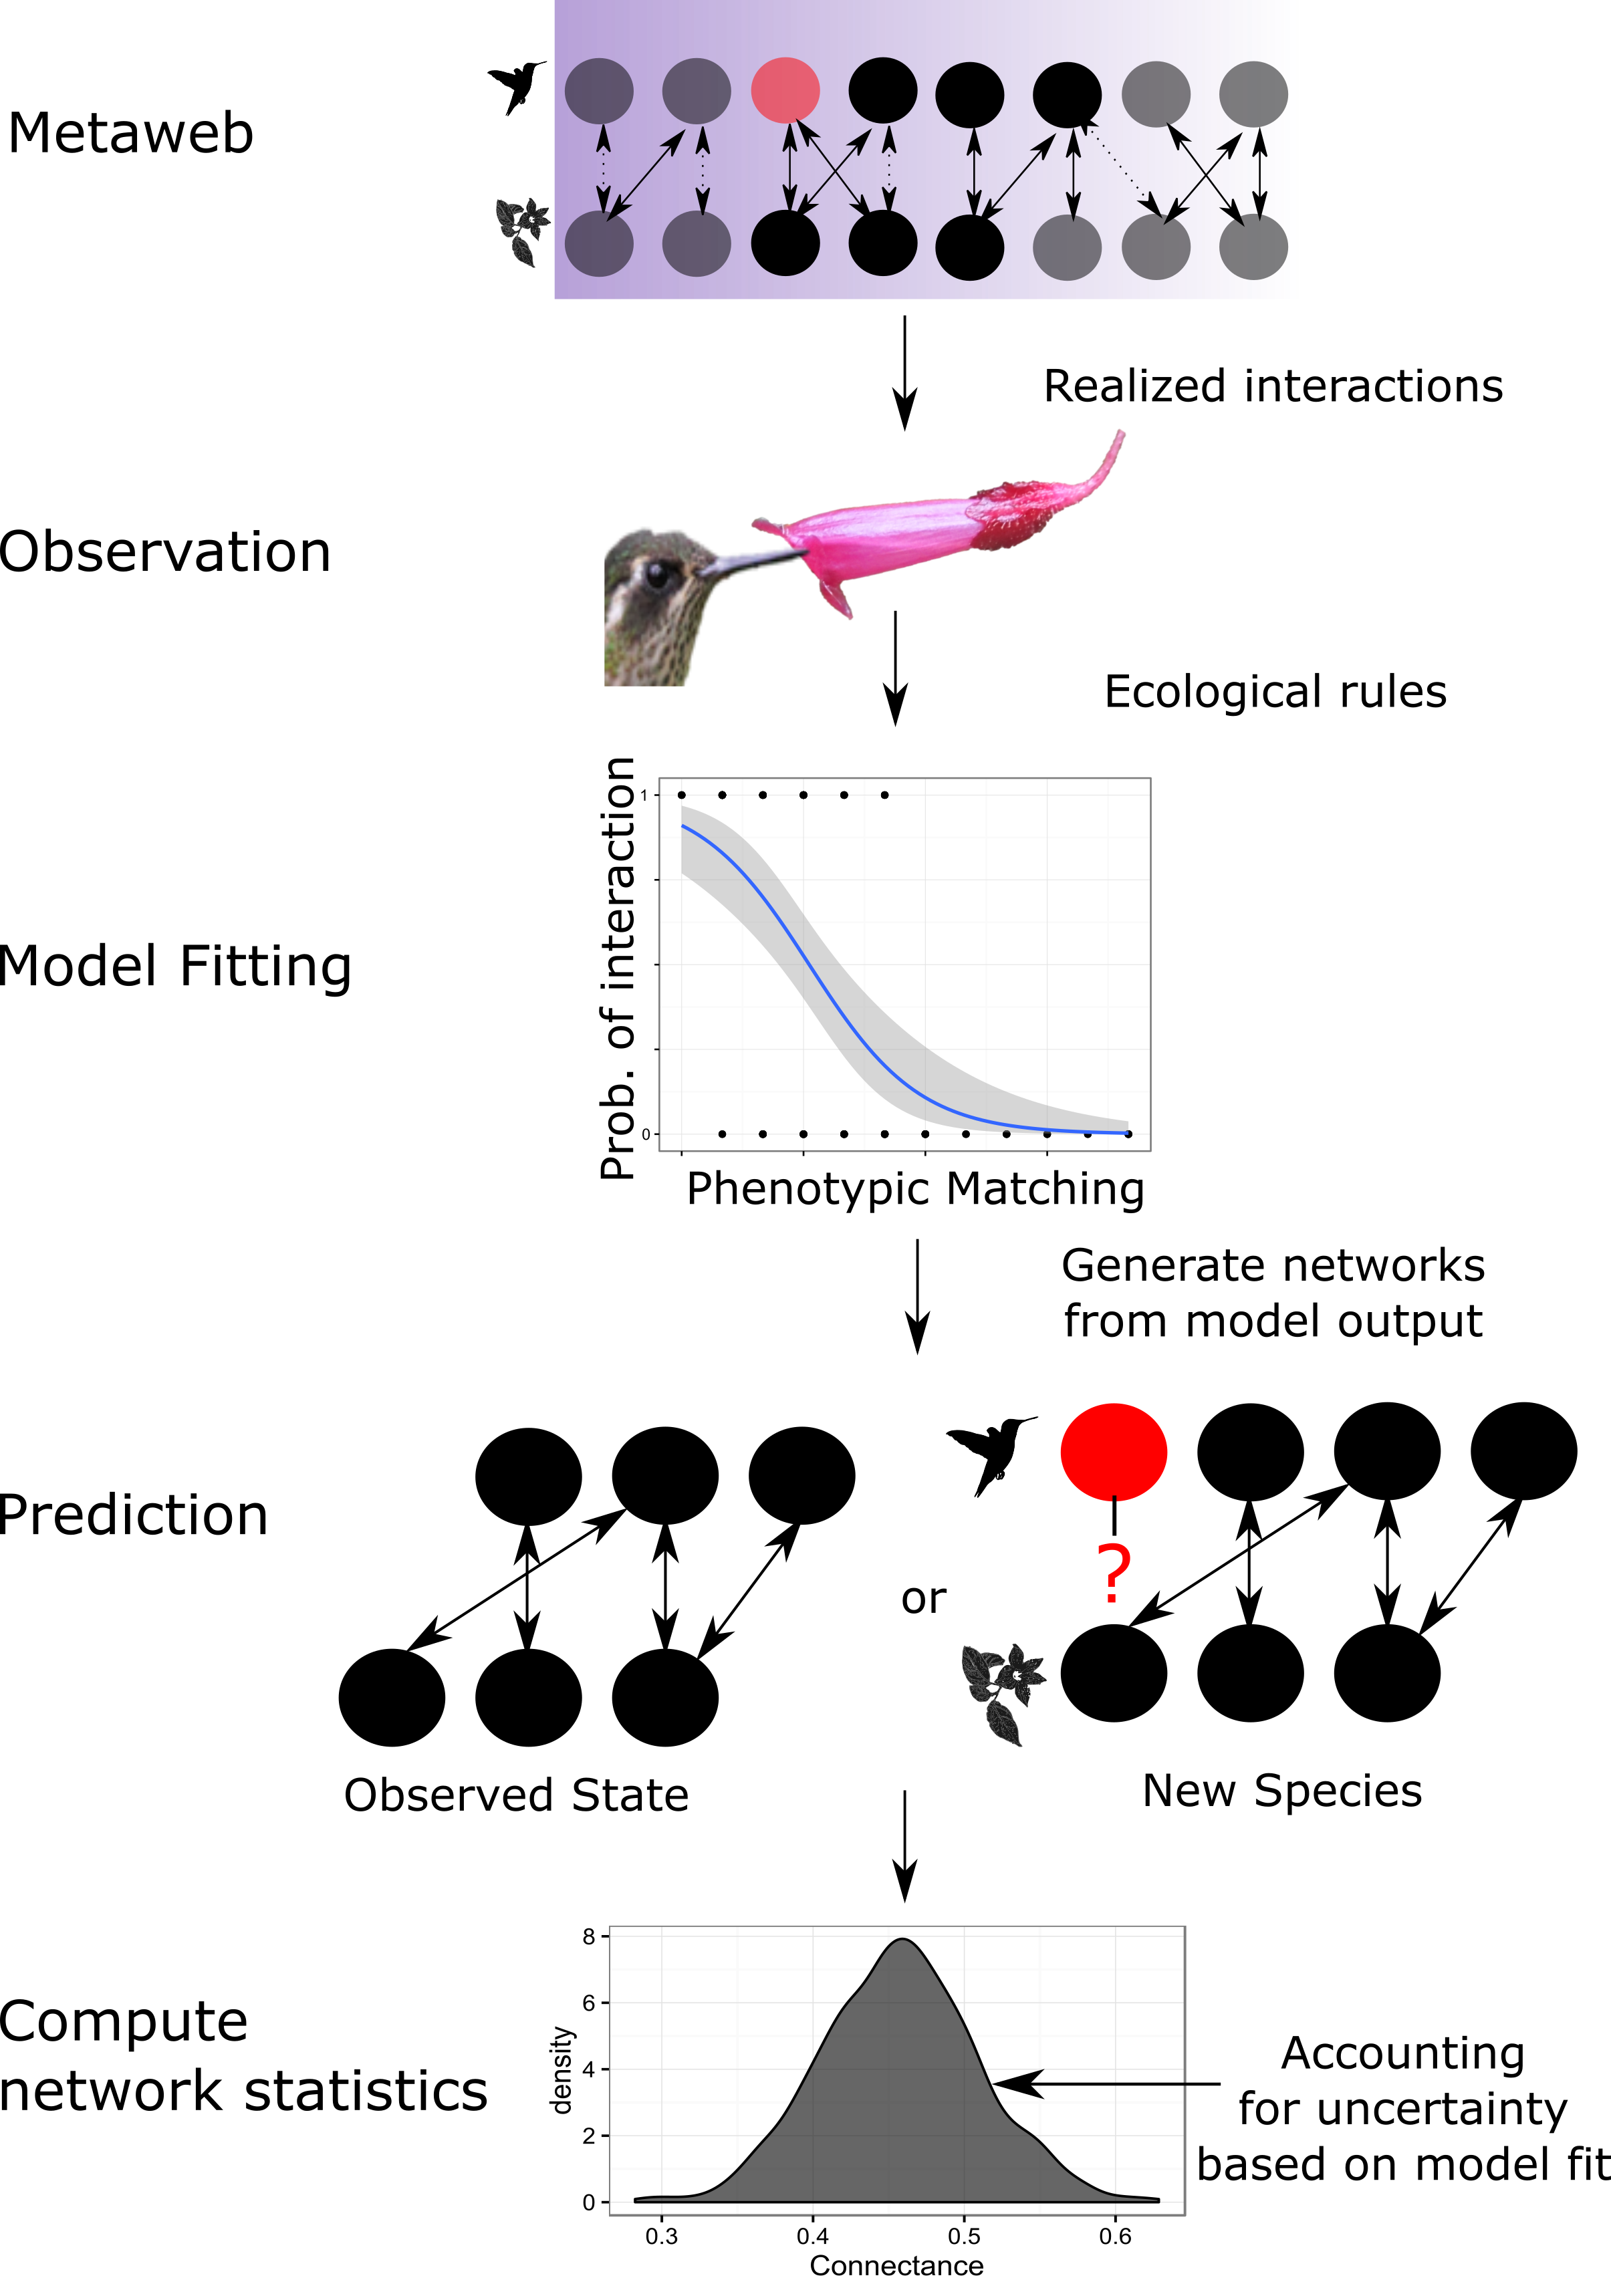
\includegraphics[width=\linewidth]{Figures/ConceptualFigure.png}
  \caption{Conceptual outline of using models to estimate species
  interactions}
  \label{fig:concept}
\end{figure}


\begin{sidewaystable}
\centering
\caption{Methods compared and how they apply}
\label{comparisonTab}
\begin{tabular}{llccccccccccc}
                                                & \multicolumn{5}{c}{Input Data}                                                                                                                                         & \multicolumn{1}{c}{}              & \multicolumn{1}{c}{}              & \multicolumn{1}{c}{}           & \multicolumn{1}{c}{}       & \multicolumn{1}{c}{}                   & \multicolumn{1}{c}{}                                                                                                                     \\
                                                & \multicolumn{1}{c}{abundance} & \multicolumn{1}{c}{Indirect  knowledge} & \multicolumn{1}{c}{Co-occurence} & \multicolumn{1}{c}{Trait} & \multicolumn{1}{c}{Phylogeny} & \multicolumn{1}{c}{Theory-driven} & \multicolumn{1}{c}{Type of links} & \multicolumn{1}{c}{Predictive} & \multicolumn{1}{c}{Output} & \multicolumn{1}{c}{Hypothesis testing} & \multicolumn{1}{c}{Example}                                                                                                              \\
Fourth-corner                                   & x                             &                                         &                                  & x                         &                               & yes                               & quantitative                      & mecanistic                     &                            &                                        & \begin{tabular}[c]{@{}l@{}}I\_eat (Beauschene et al. 2016)\\ Markov logic, Intuitive Logic Programming (Vacher et al. 2016)\end{tabular} \\
Maching learning                                & x                             & x                                       & (x)                              & (x)                       & (x)                           & no                                & quantitative                      & data-based                     &                            &                                        & Rohr et al. 2014, Rohr et al. 2016                                                                                                       \\
Direct mathcing-centrality                      &                               &                                         &                                  & x                         & x                             & yes                               & quantitative                      & mecanistic                     &                            &                                        &                                                                                                                                          \\
Indirect matching-centrality                    &                               &                                         &                                  &                           &                               &                                   &                                   &                                &                            &                                        &                                                                                                                                          \\
Niche model                                     &                               &                                         &                                  &                           &                               &                                   &                                   &                                &                            &                                        &                                                                                                                                          \\
Hierarchical model                              &                               &                                         &                                  &                           &                               &                                   &                                   &                                &                            &                                        &                                                                                                                                          \\
Null model                                      &                               &                                         &                                  &                           &                               &                                   &                                   &                                &                            &                                        &                                                                                                                                          \\
Joint Spatial Division and Multiplexing (JSDM)  &                               &                                         &                                  &                           &                               &                                   &                                   &                                &                            &                                        &                                                                                                                                          \\
Intercept                                       &                               &                                         &                                  &                           &                               &                                   &                                   &                                &                            &                                        &                                                                                                                                          \\
GLM/cooccur                                     &                               &                                         &                                  &                           &                               &                                   &                                   &                                &                            &                                        &                                                                                                                                          \\
Grouping species into nodes (functional groups) &                               & x                                       &                                  & x                         &                               & no                                & Binary (quantitative)             & no                             &                            &                                        &                                                                                                                                          \\
Expert-based assesment of links                 &                               & x                                       &                                  & x                         &                               & no                                & Binary (quantitative)             & no                             &                            &                                        &
\end{tabular}
\end{sidewaystable}



\end{document}
